% Beamer Presentation and Lecture Note Template
% Version 0.1
% by Paul Vesey

\mode<presentation> {
\usetheme{Antibes}
\setbeamercovered{invisible}
\setbeamertemplate{footline}[frame number]
\setbeamertemplate{navigation symbols}{} 
}

\usepackage{eurosym}
\usepackage{graphicx}
\usepackage{wasysym}
\usepackage{hyperref}
\usepackage{amsmath}
\usepackage{amssymb}
\usepackage{mathtools}
\usepackage{tikz}
\usepackage{pgf}
\usepackage{pgfplots}
\usepackage{pxfonts}
\usepackage{textcomp}
\usepackage{verbatim}
\usepackage{color}
\usepackage{xcolor}
\usepackage{fix-cm}


\author{Paul Vesey}
\institute[LIT]
{
Limerick Institute of Technology \\
\medskip
{\emph{paul.vesey@lit.ie}}
}
\date{2016-2017}



%\usepackage{bm} 
% For typesetting bold math (not \mathbold)
%\logo{\includegraphics[height=0.6cm]{yourlogo.eps}}
%
\title[Introduction to Project Management]{Introduction to Project Management}


\begin{document}
%
\usetikzlibrary{arrows}
\usepgflibrary{patterns}



\thispagestyle{empty} % Remove page numbering on this page

%----------------------------------------------------------------------------------------
%	TITLE SECTION
%----------------------------------------------------------------------------------------

\hrule

\vspace*{0.7cm} % Space between the start of the title and the top of the grey box


\begin{flushright}
\Huge Services Strategy for Interior Design \\
\vspace*{0.7cm}
\Large BA in Interior Design & Technology\\
Year 2 (2016-2017)
\end{flushright}

\vspace*{0.7cm} % Space between the end of the title and the bottom of the grey box
	
\normalsize

\hrule

%----------------------------------------------------------------------------------------

\vfill % Space between the title box and author information

%----------------------------------------------------------------------------------------
%	AUTHOR NAME AND INFORMATION SECTION
%----------------------------------------------------------------------------------------

{\centering \large 
\hfill Paul Vesey, \scriptsize BEng (Hons), MIE, HDip\normalsize \\
\hfill Limerick Institute of Technology \\
\hfill Department of the Built Environment \\
\hfill \texttt{https://paulvesey.wordpress.com} \\
\vspace*{0.7cm} 
\hrule} % Horizontal line, thickness changed here

%----------------------------------------------------------------------------------------

\clearpage % Whitespace to the end of the page

\newpage




\thispagestyle{empty}
\tableofcontents
\newpage
\section{Introduction}


\begin{frame}
\titlepage
\end{frame}\begin{center}\line(1,0){250}\end{center}
%
%
\begin{center}\line(1,0){250}\end{center}



\begin{frame}
\frametitle{Introduction to Lighting}
\textbf{Mathematics and Units}
\begin{itemize}
	\item Most useful SI unit is \textbf{lux} (lx). 1 lux is 1 lumen/m2
	\item lx is a measure of luminance and emittance
	\item Working lux levels from the sun are about 4,000 lx in Ireland and about 11,000 in Dubai
	\item Light Intensity follows the inverse square law
\end{itemize}

\begin{center}
$Intensity = \frac{1}{distance^2}$
\end{center}

\end{frame}
\begin{center}\line(1,0){250}\end{center}




\begin{frame}
\frametitle{Introduction to Lighting}
	\begin{table}
		\centering
			\begin{tabular}{|l|r|}
				\hline
				Condition 			& Illumination (lx)\\
				\hline
				Sunlight 				&	107,527\\
				Full Daylight 	&	10,752\\
				Overcast Day 		&	1,075\\
				Very Dark Day 	&	107\\
				Twilight 				&	10.8\\
				Deep Twilight 	&	1.08\\
				Full Moon 			&	0.108\\
				Quarter Moon 		&	0.0108\\
				Starlight 			&	0.0011\\
				Overcast Night 	&	0.0001\\
				\hline
			\end{tabular}
	\end{table}
\end{frame}
\begin{center}\line(1,0){250}\end{center}








\begin{frame}
\frametitle{Introduction to Lighting}
	\begin{table}
		\centering
			\scalebox{0.65}{
			\begin{tabular}{|l|r|}
				\hline
				\textbf{Activity}  & \textbf{Illumination} (lx)\\
				\hline
					Public areas with dark surroundings &20 - 50\\\hline
					Simple orientation for short visits &50 - 100\\\hline
					Working areas where visual tasks are & \\
					only occasionally performed &100 - 150\\\hline
					Warehouses, Homes, Theaters, Archives &150\\\hline
					Easy Office Work, Classes &250\\\hline
					Normal Office Work, PC Work, Study Library, &\\
					Groceries, Show Rooms, Laboratories &500\\\hline
					Supermarkets, Mechanical Workshops, Office Landscapes &750\\\hline
					Normal Drawing Work, Detailed Mechanical Workshops, &\\
					Operation Theatres &1,000\\\hline
					Detailed Drawing Work, Very Detailed Mechanical Works &1500 - 2000\\\hline
					Performance of visual tasks of low contrast  &\\
					and very small size for prolonged periods of time &2000 - 5000\\\hline
					Performance of very prolonged and exacting visual tasks &5000 - 10000\\\hline
					Performance of very special visual tasks of &\\
					extremely low contrast and small size &10000 - 20000\\\hline
				\hline
			\end{tabular}
			}
	\end{table}
\end{frame}
\begin{center}\line(1,0){250}\end{center}




\begin{frame}
\frametitle{Types of Lighting}
\begin{itemize}
	\item Ambient (normal lighting)
	\item Task (reading, assembly, etc.)
	\item	Accent (used to create visual interest)
\end{itemize}
Read more: \href{https://www.americanlightingassoc.com/}{https://www.americanlightingassoc.com/}
\end{frame}
\begin{center}\line(1,0){250}\end{center}




\begin{frame}
\frametitle{Daylighting and Artificial Lighting}
\begin{itemize}
	\item In the past many designers only used Artificial Lighting; easier to control and design
	\item Sustainability requirements have led to the reemergence of Day-lighting solutions, but requires careful design
\end{itemize}
Analysis tools can typically handle both types quite well.
\end{frame}
\begin{center}\line(1,0){250}\end{center}


\begin{frame}
\frametitle{Artificial Lighting \hfill\hfill Lamps}
\begin{itemize}
	\item Commonly called “bulbs”. Unprofessional; Pro’s call them \textbf{lamps}.
	\item \textbf{Incandescent} - typical lamp in common usage
	\item \textbf{Florescent} - typical “strip” light
	\item \textbf{CFL} - Compact Florescent Lamp, commonly called “low energy bulbs”
	\item \textbf{LED} - Light Emitting Diode, typically many LEDs and circuitry in one lamp
	\item \textbf{HID} - High Intensity Discharge (typically gas filled)
\end{itemize}
\end{frame}
\begin{center}\line(1,0){250}\end{center}


\begin{frame}
\frametitle{Artificial Lighting \hfill\hfill Luminaires}
\begin{itemize}
	\item Technical term for light fittings
	\item Have a profound effect on the characteristics of light emitted
	\item Also have a profound effect on the overall aesthetic of the interior design
\end{itemize}
Read more: \href{http://www.lightingproducts.philips.com/}{http://www.lightingproducts.philips.com/}
\end{frame}
\begin{center}\line(1,0){250}\end{center}



\begin{frame}
\frametitle{Luminaires \hfill\hfill Technical Characteristics}
\begin{figure}
	\centering
		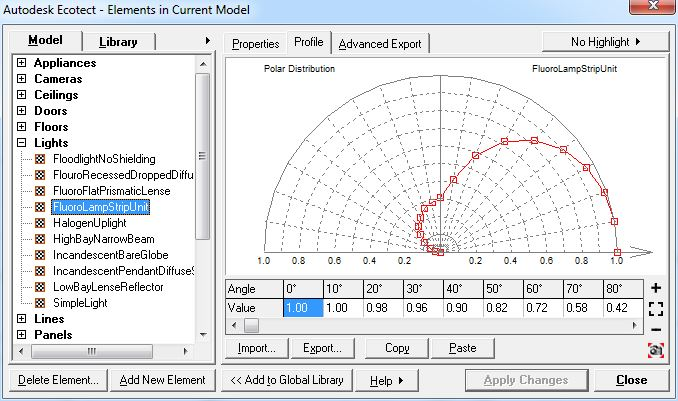
\includegraphics[width=8cm]{../img/lumTechSpec.jpg}
	\caption{Autodesk Ecotect Luminaire}
	\label{fig:lumTechSpec}
\end{figure}
\end{frame}
\begin{center}\line(1,0){250}\end{center}


\begin{frame}
\frametitle{Luminaires \hfill\hfill Types}
\begin{figure}
	\centering
		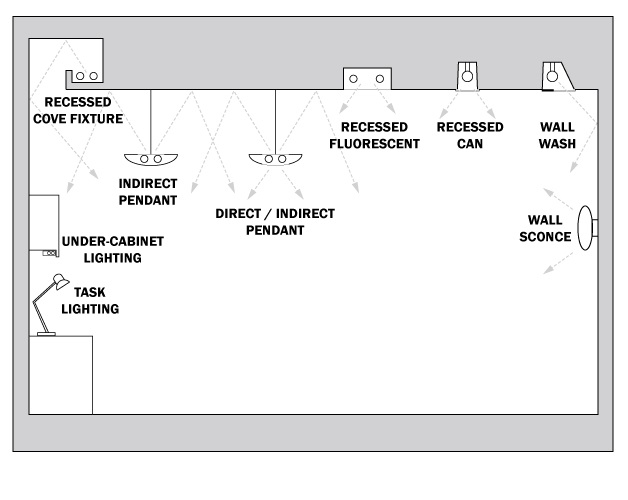
\includegraphics[width=8cm]{../img/lightingtypes.jpg}
	\caption{Luminaire Types}
	\label{fig:lightingtypes}
\end{figure}

\end{frame}
\begin{center}\line(1,0){250}\end{center}



\end{document}
